\begin{frame}
\frametitle{SSH-based detection}
\begin{figure}
	\centering
% 	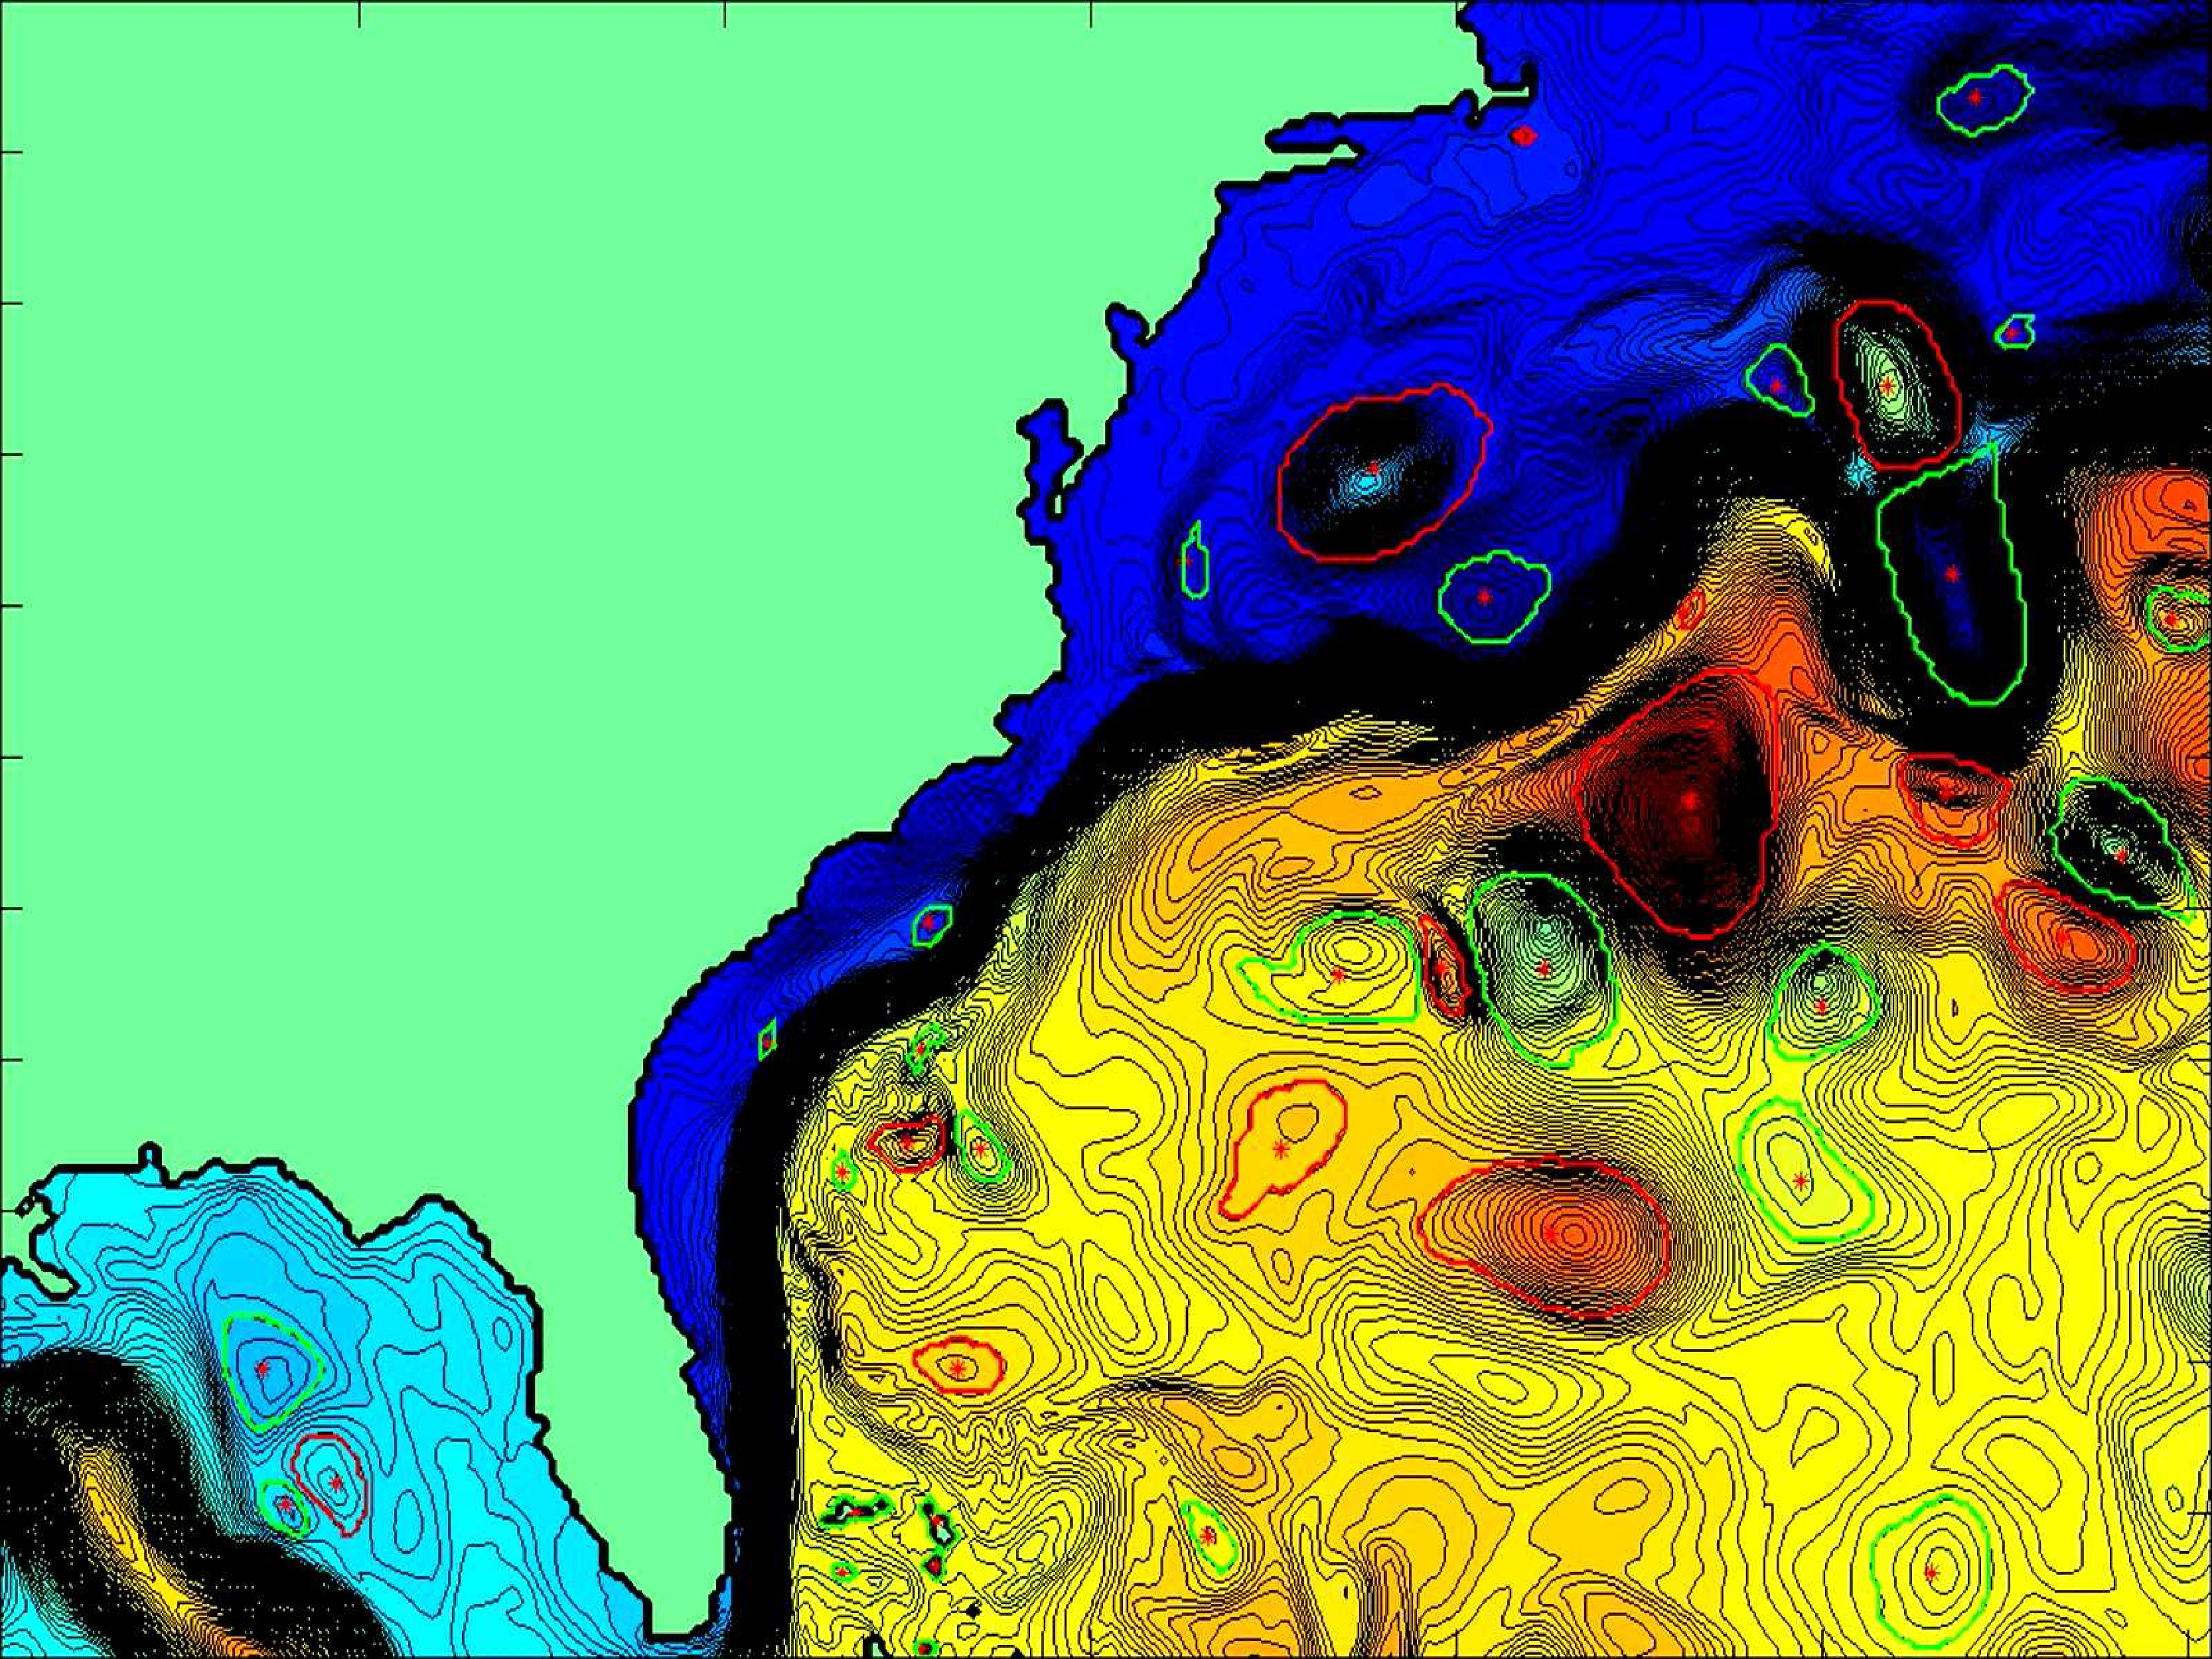
\includegraphics[width=300pt,keepaspectratio=true]{GS.pdf}
	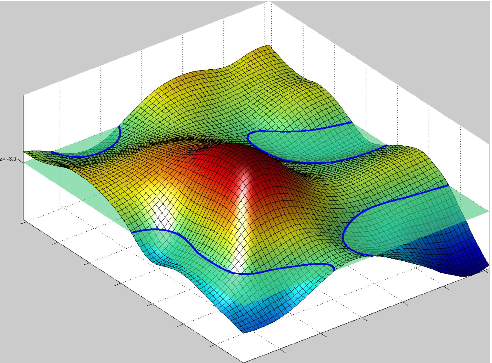
\includegraphics[height=200pt,keepaspectratio=true]{shrunks/slice1.pdf}
\end{figure}
\end{frame}

\begin{frame}[noframenumbering]
\frametitle{SSH-based detection}
\begin{figure}
	\centering
% 	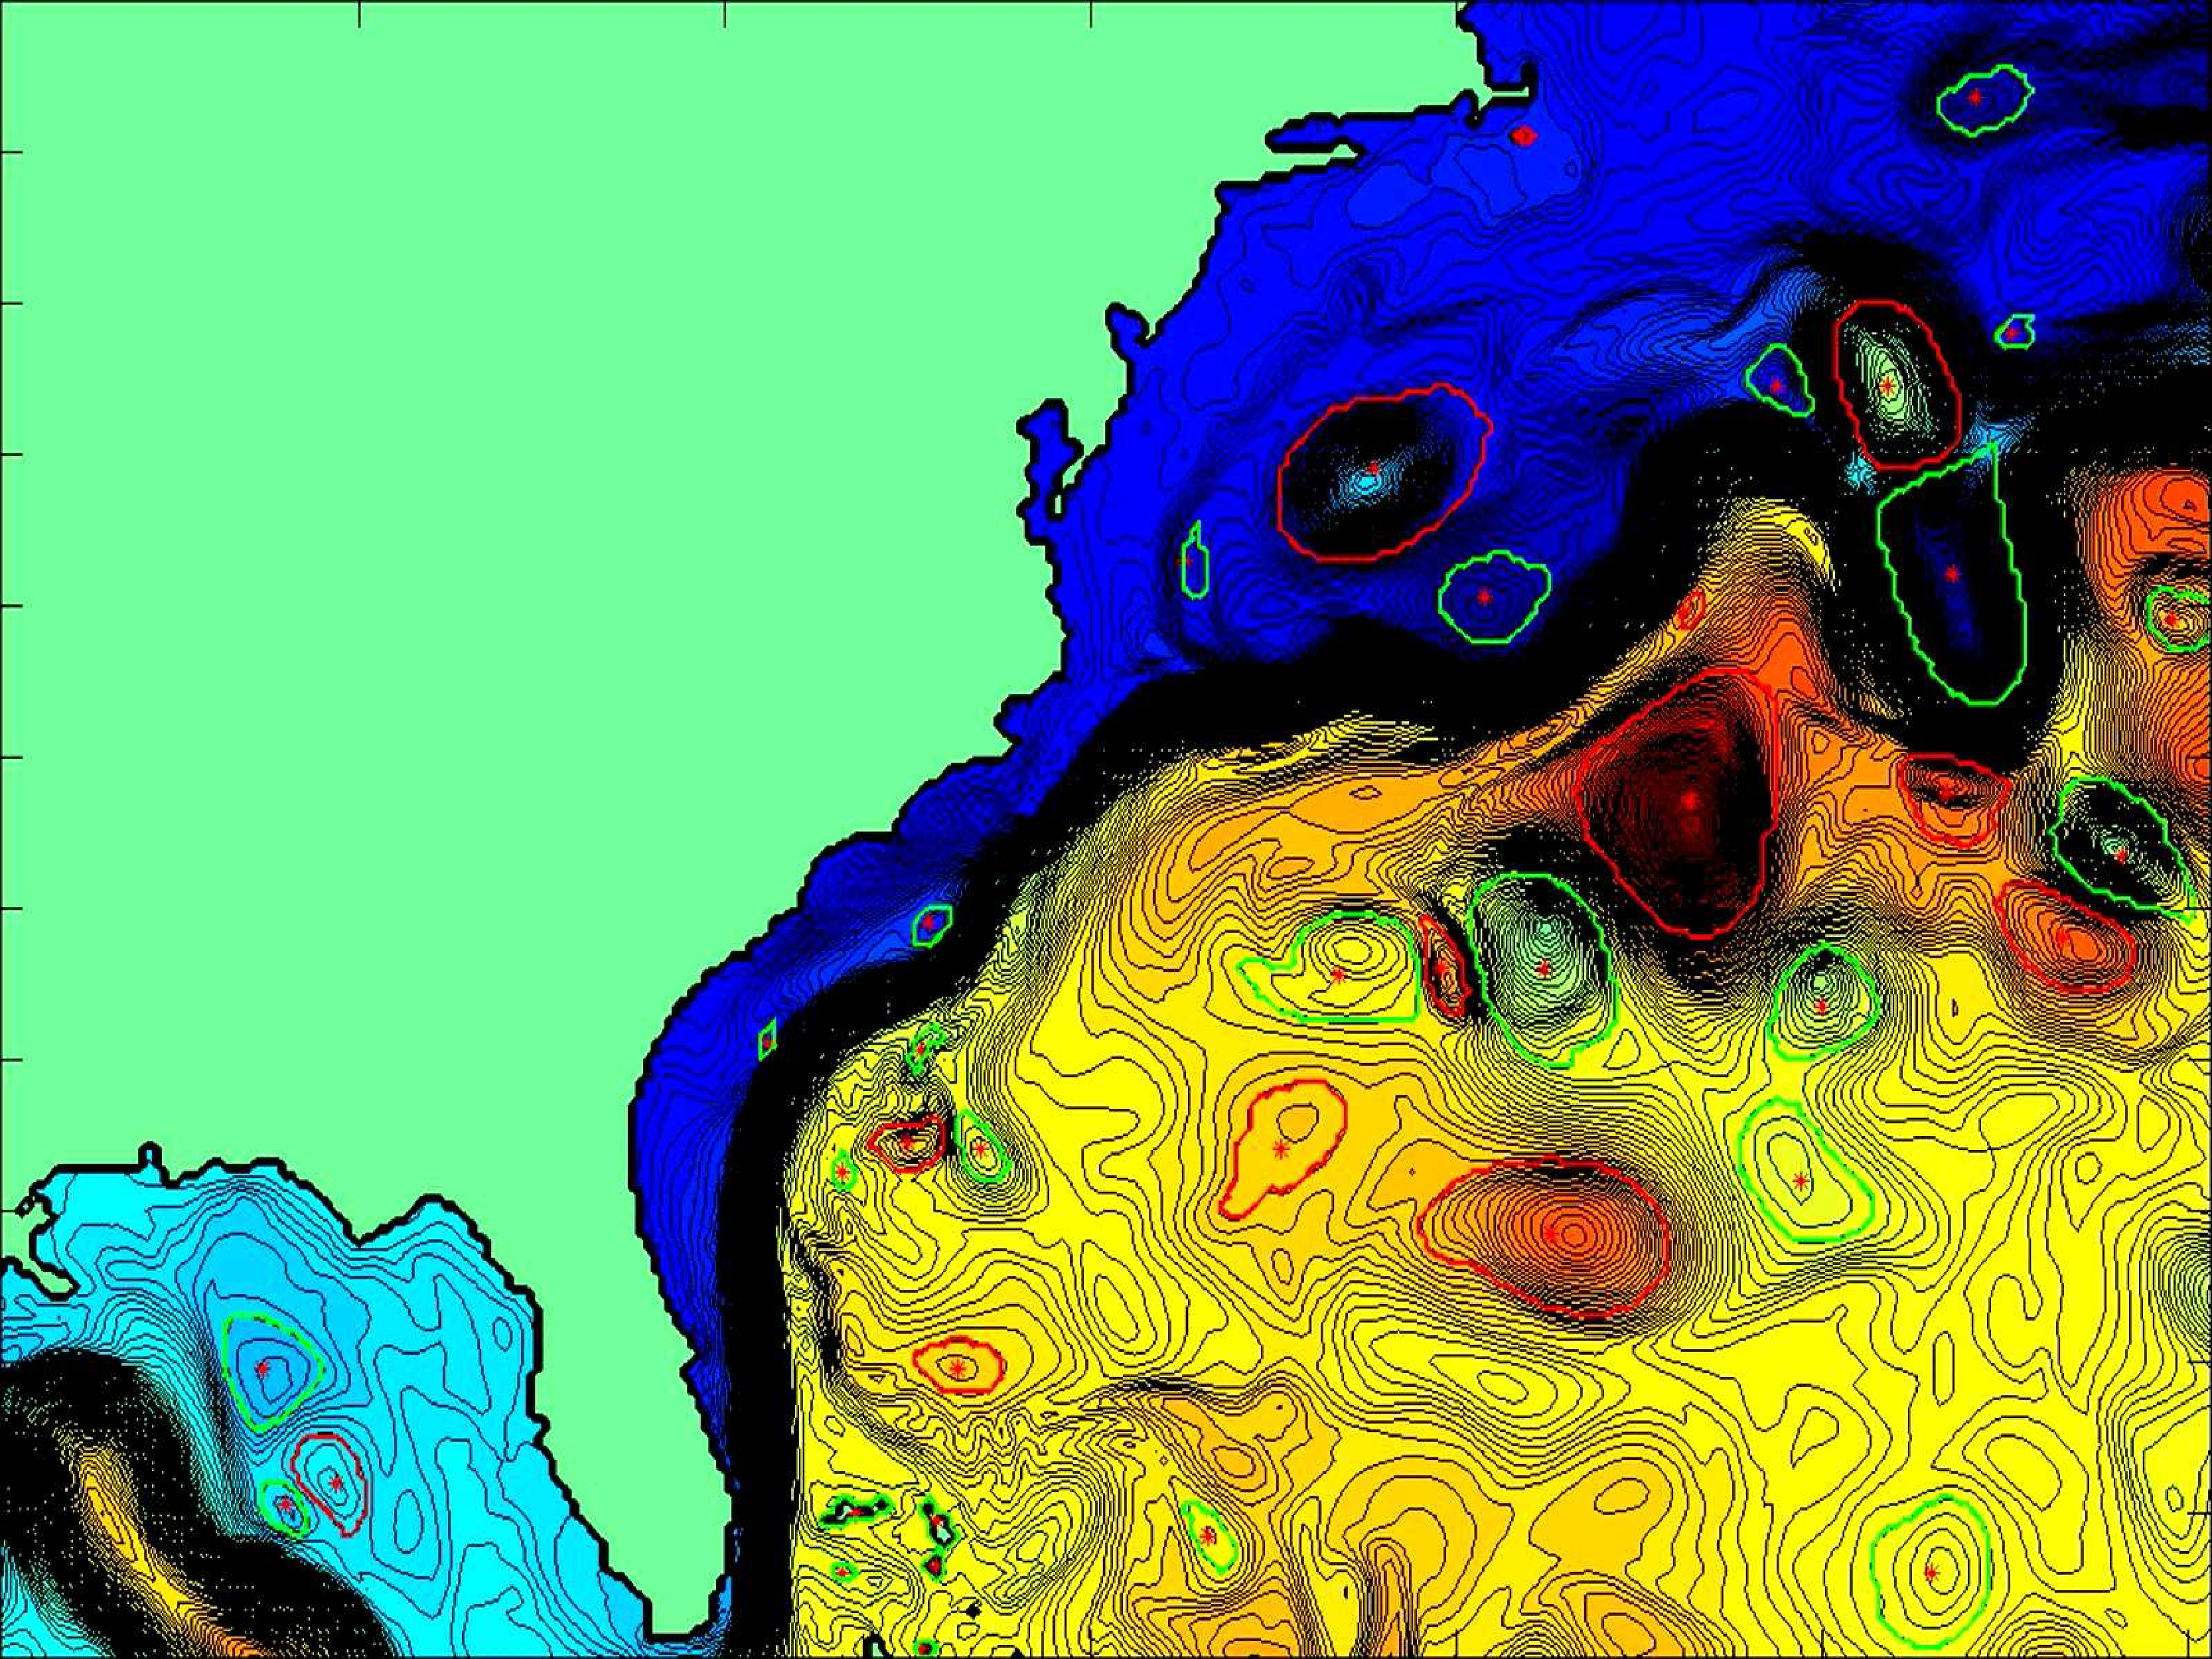
\includegraphics[width=300pt,keepaspectratio=true]{GS.pdf}
	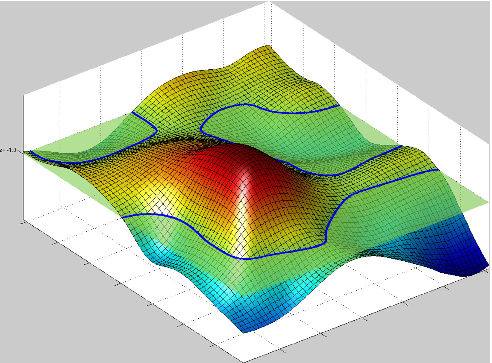
\includegraphics[height=200pt,keepaspectratio=true]{shrunks/slice2.pdf}
\end{figure}
\end{frame}

\begin{frame}[noframenumbering]
\frametitle{SSH-based detection}
\begin{figure}
	\centering
% 	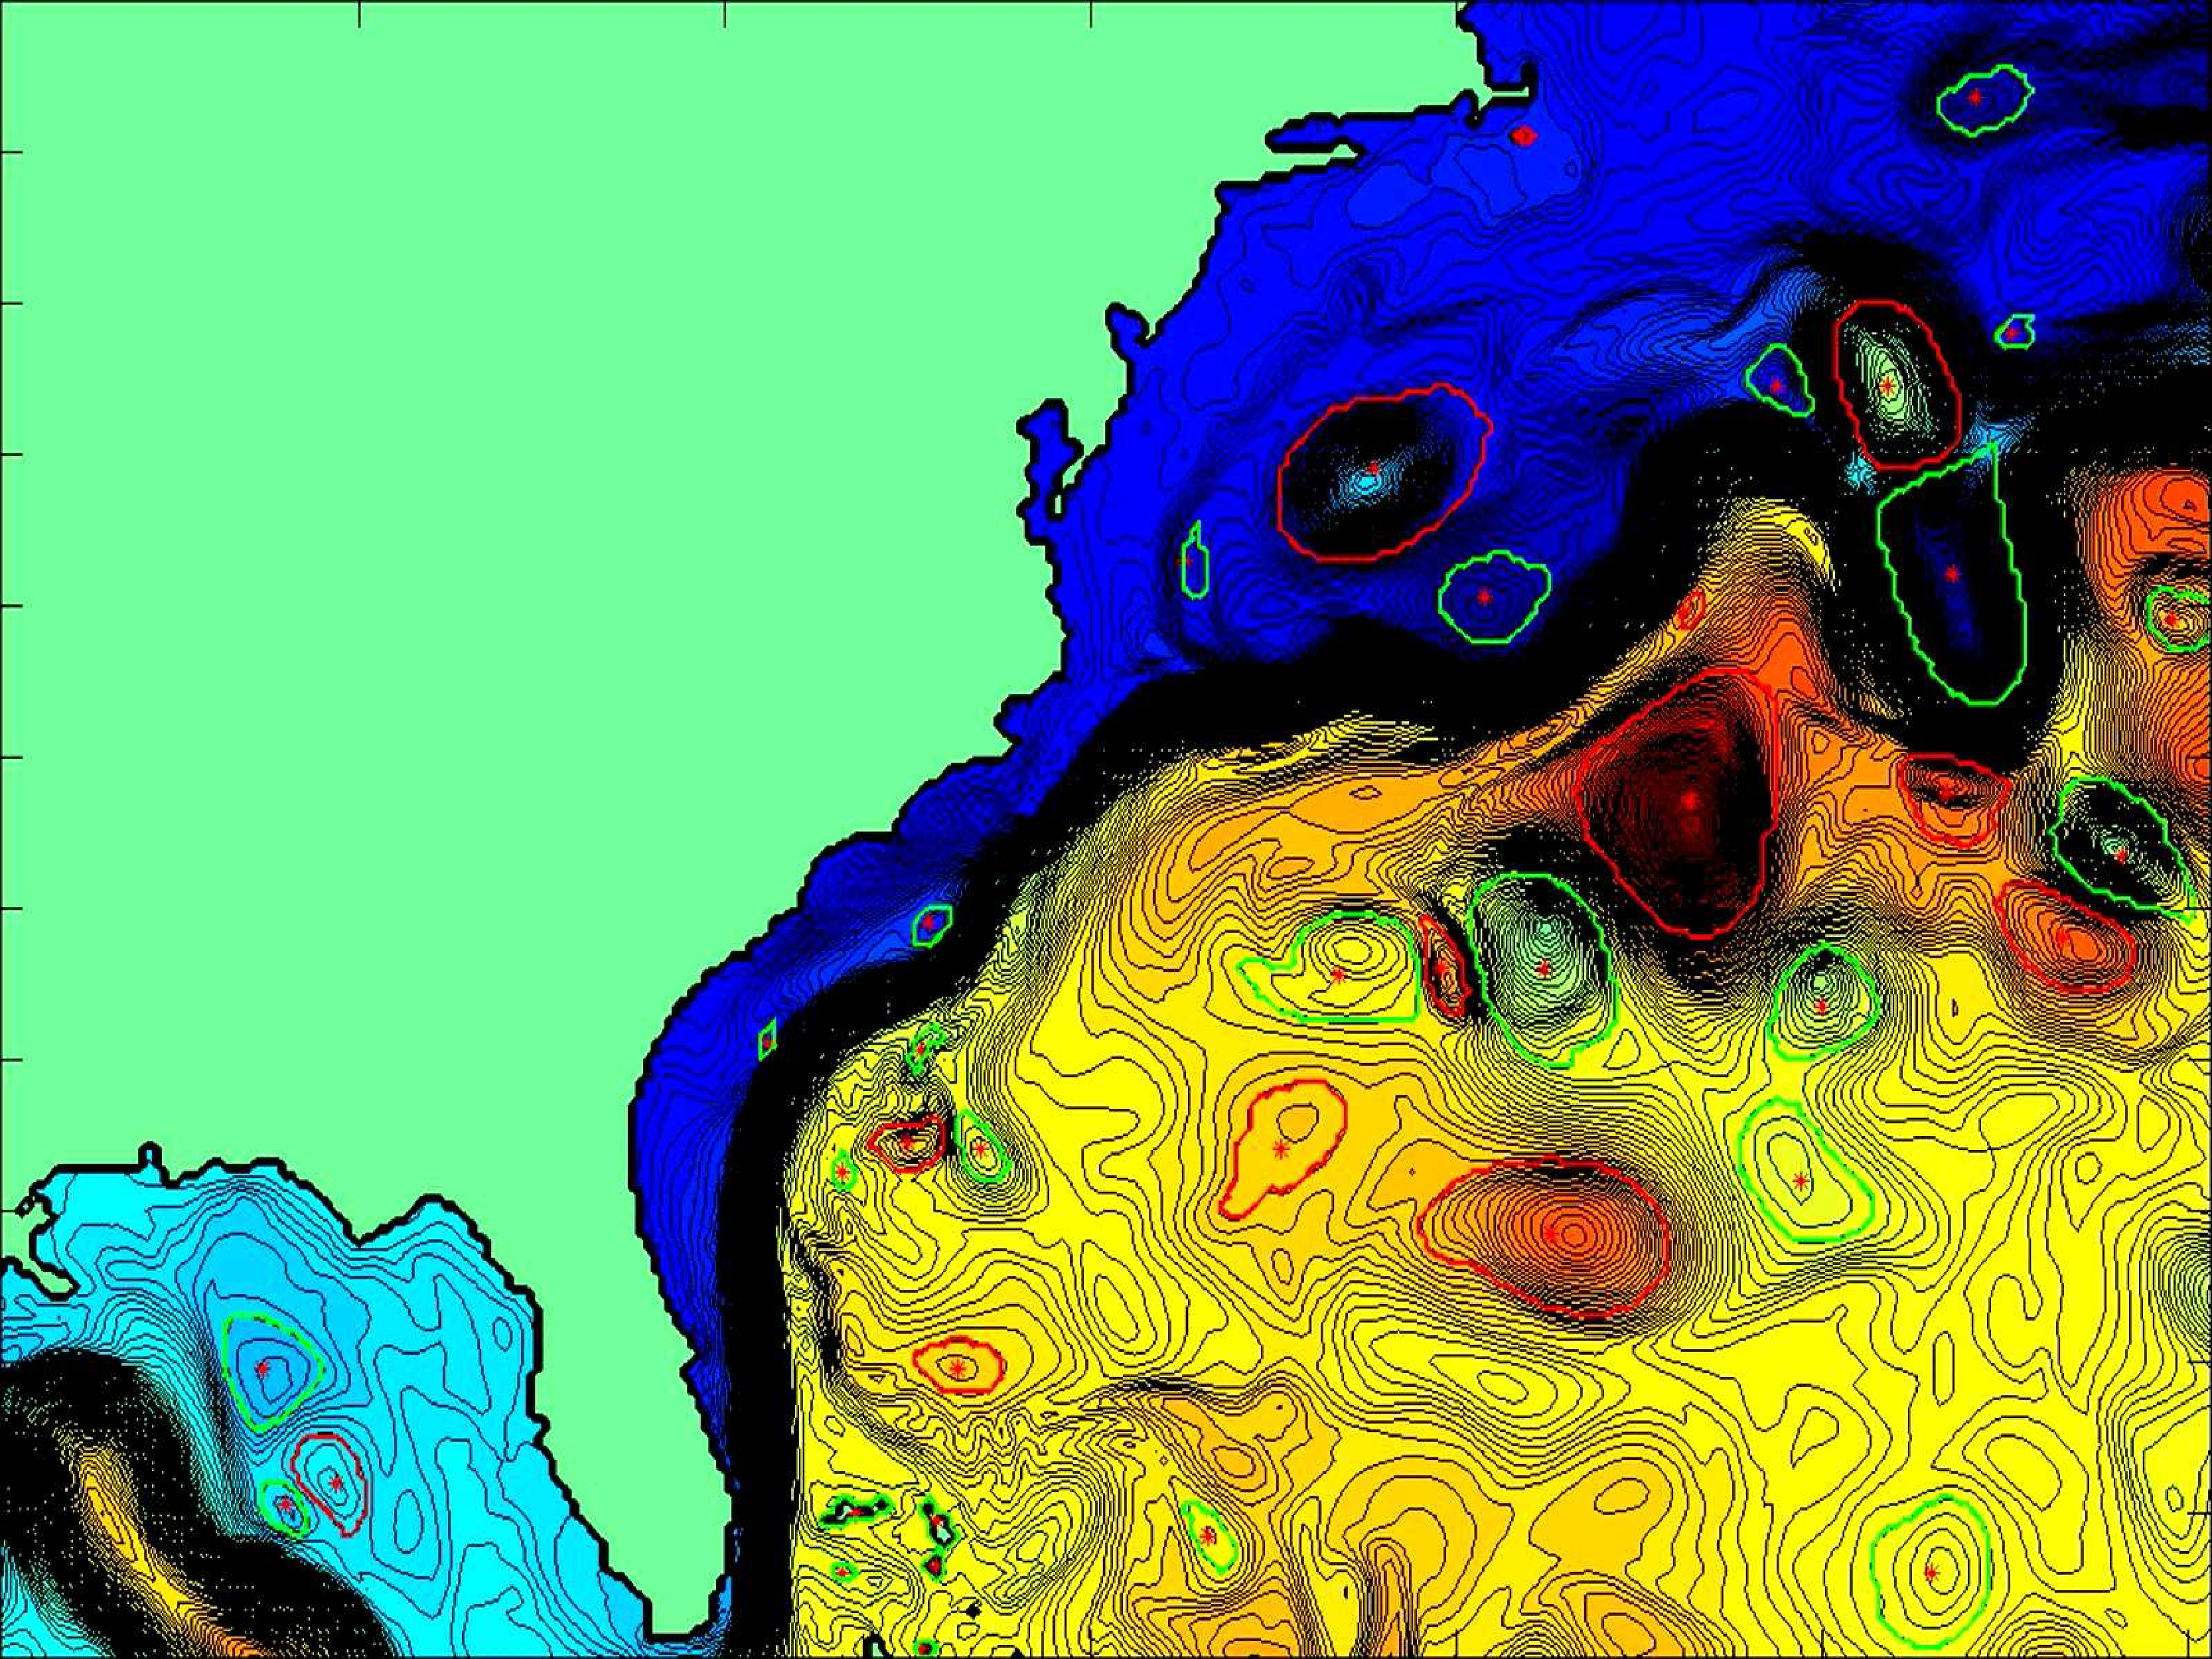
\includegraphics[width=300pt,keepaspectratio=true]{GS.pdf}
	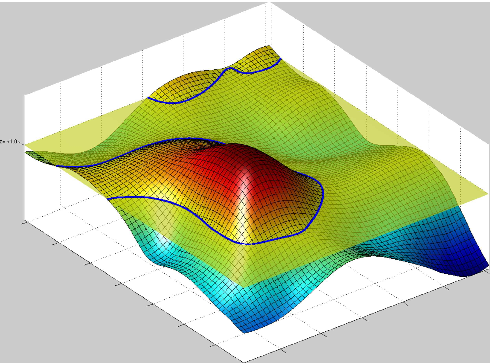
\includegraphics[height=200pt,keepaspectratio=true]{shrunks/slice3.pdf}
\end{figure}
\end{frame}

\begin{frame}[noframenumbering]
\frametitle{SSH-based detection}
\begin{figure}
	\centering
% 	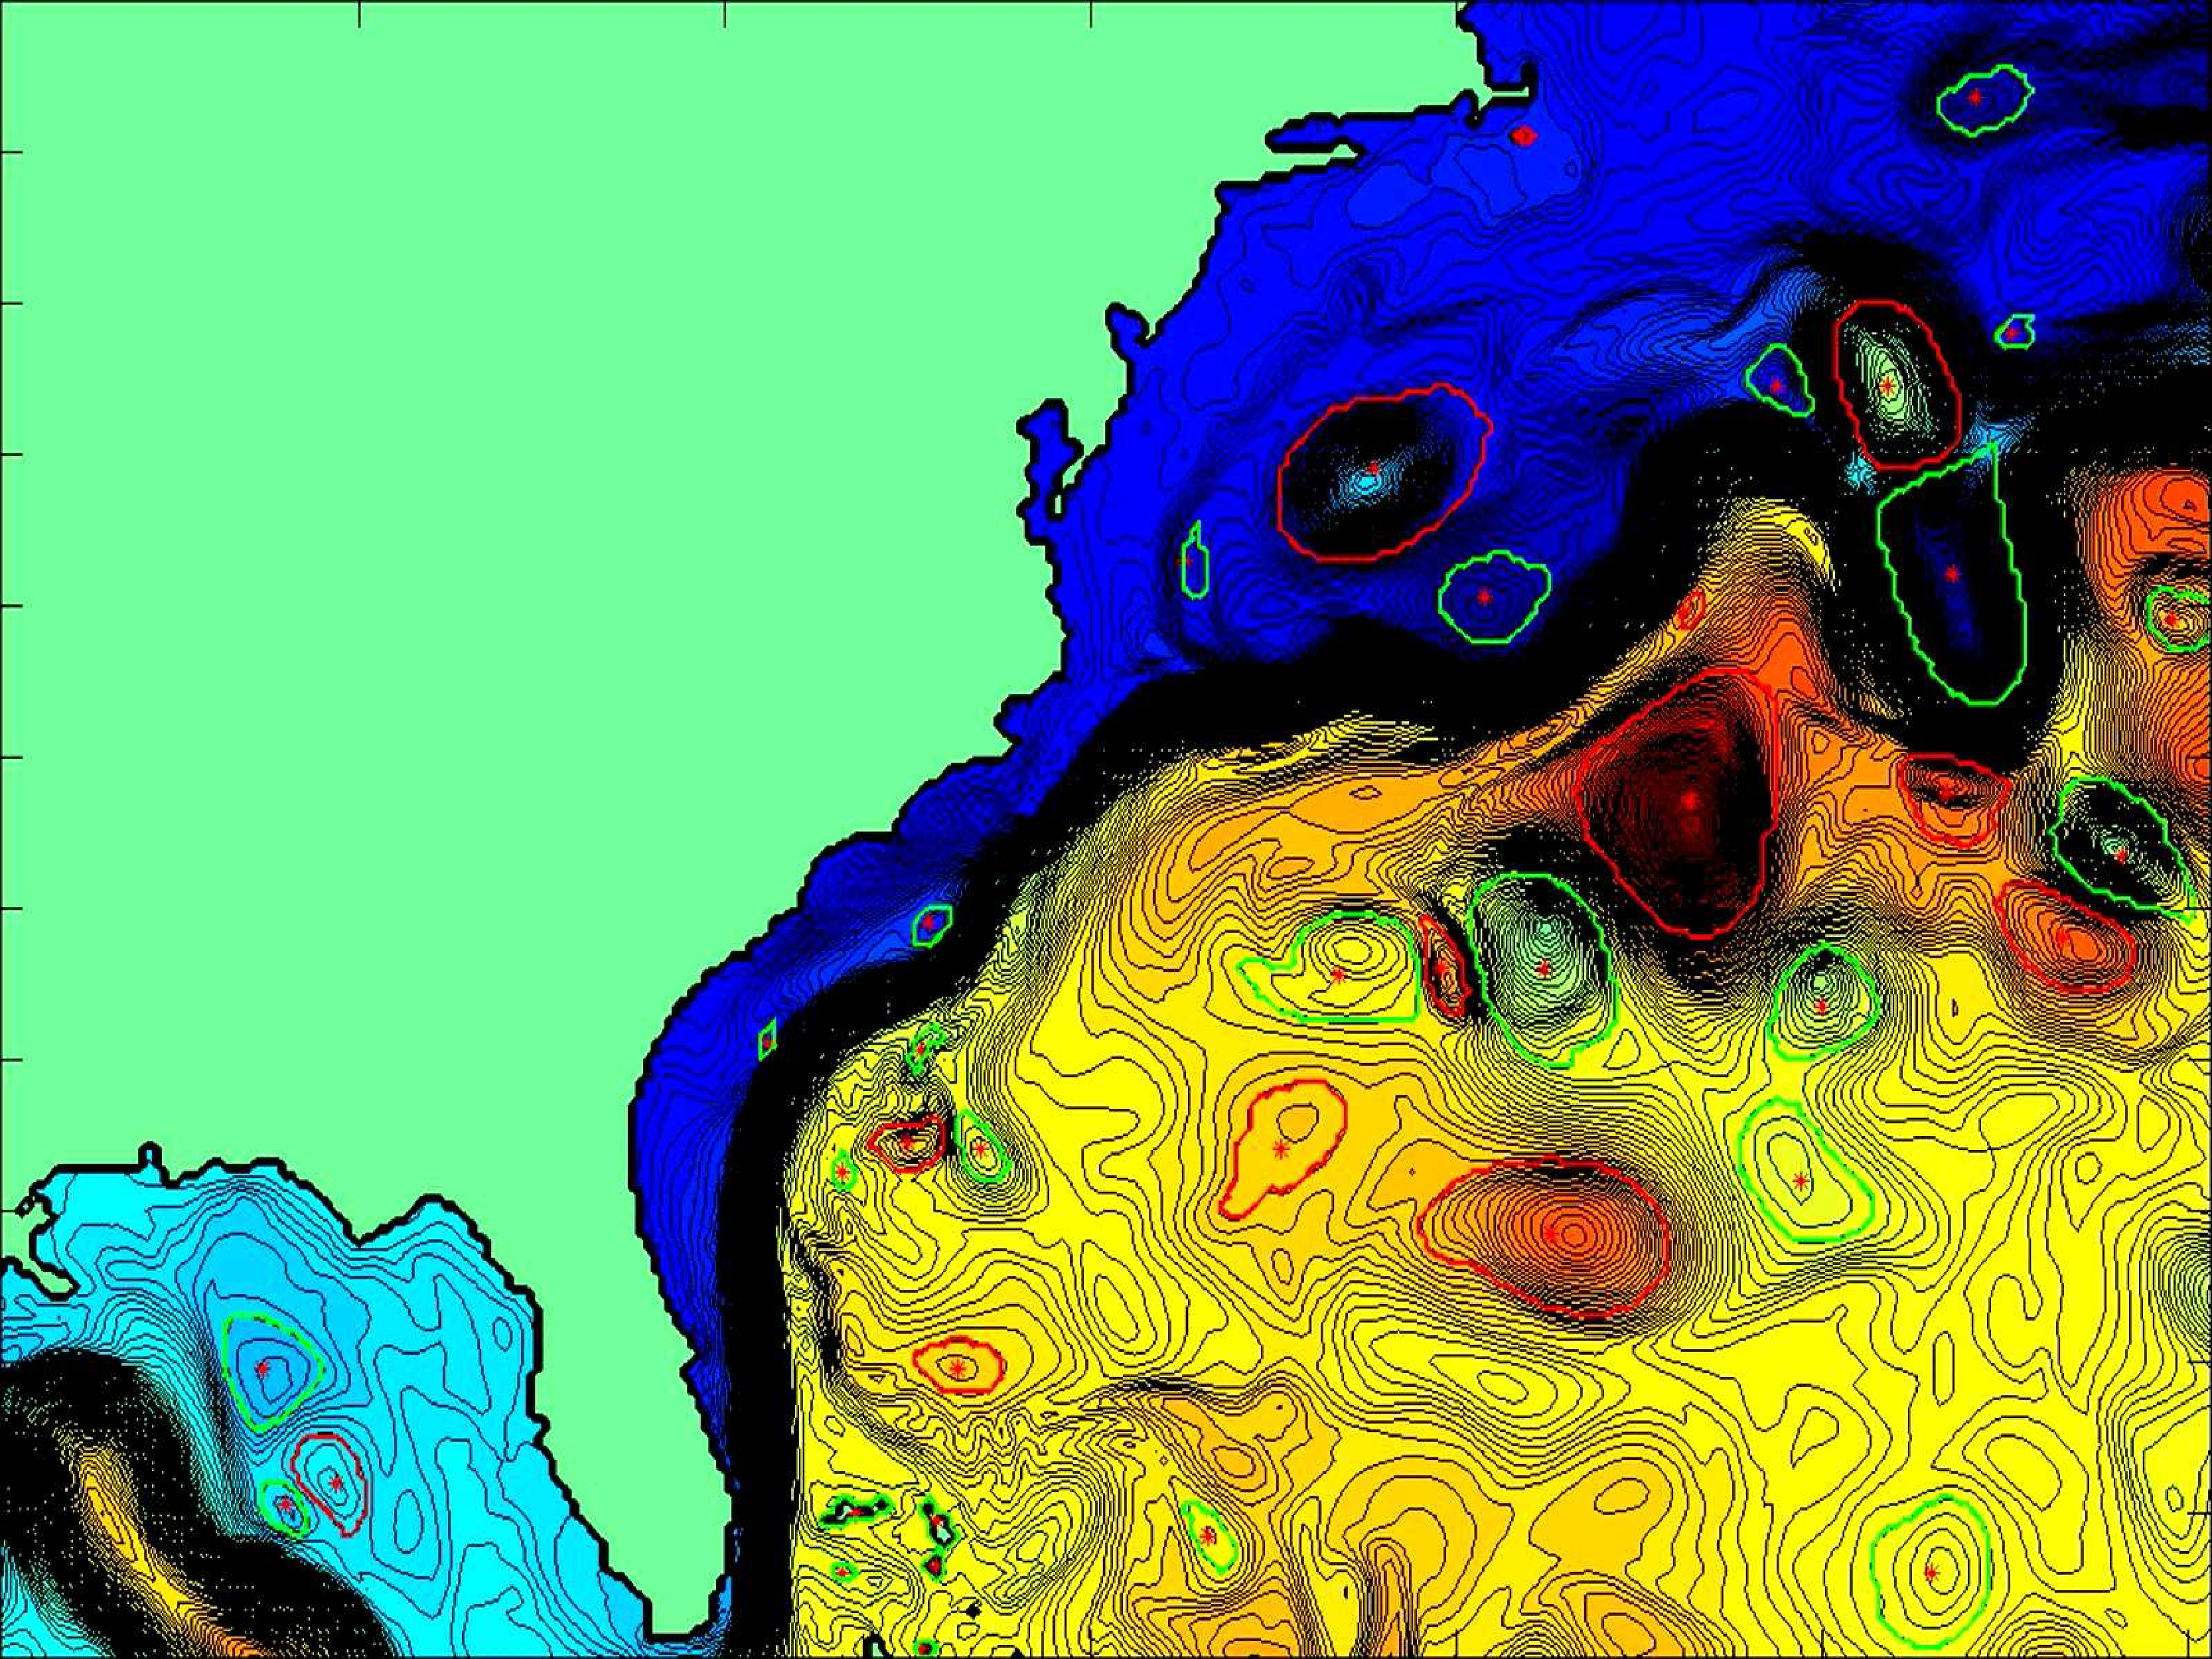
\includegraphics[width=300pt,keepaspectratio=true]{GS.pdf}
	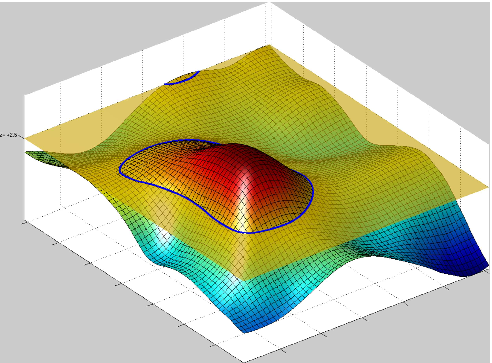
\includegraphics[height=200pt,keepaspectratio=true]{shrunks/slice4.pdf}
\end{figure}
\end{frame}

%\begin{frame}[noframenumbering]
%% \frametitle{pictures in latex beamer class}
%\begin{figure}
	%\centering
%% 	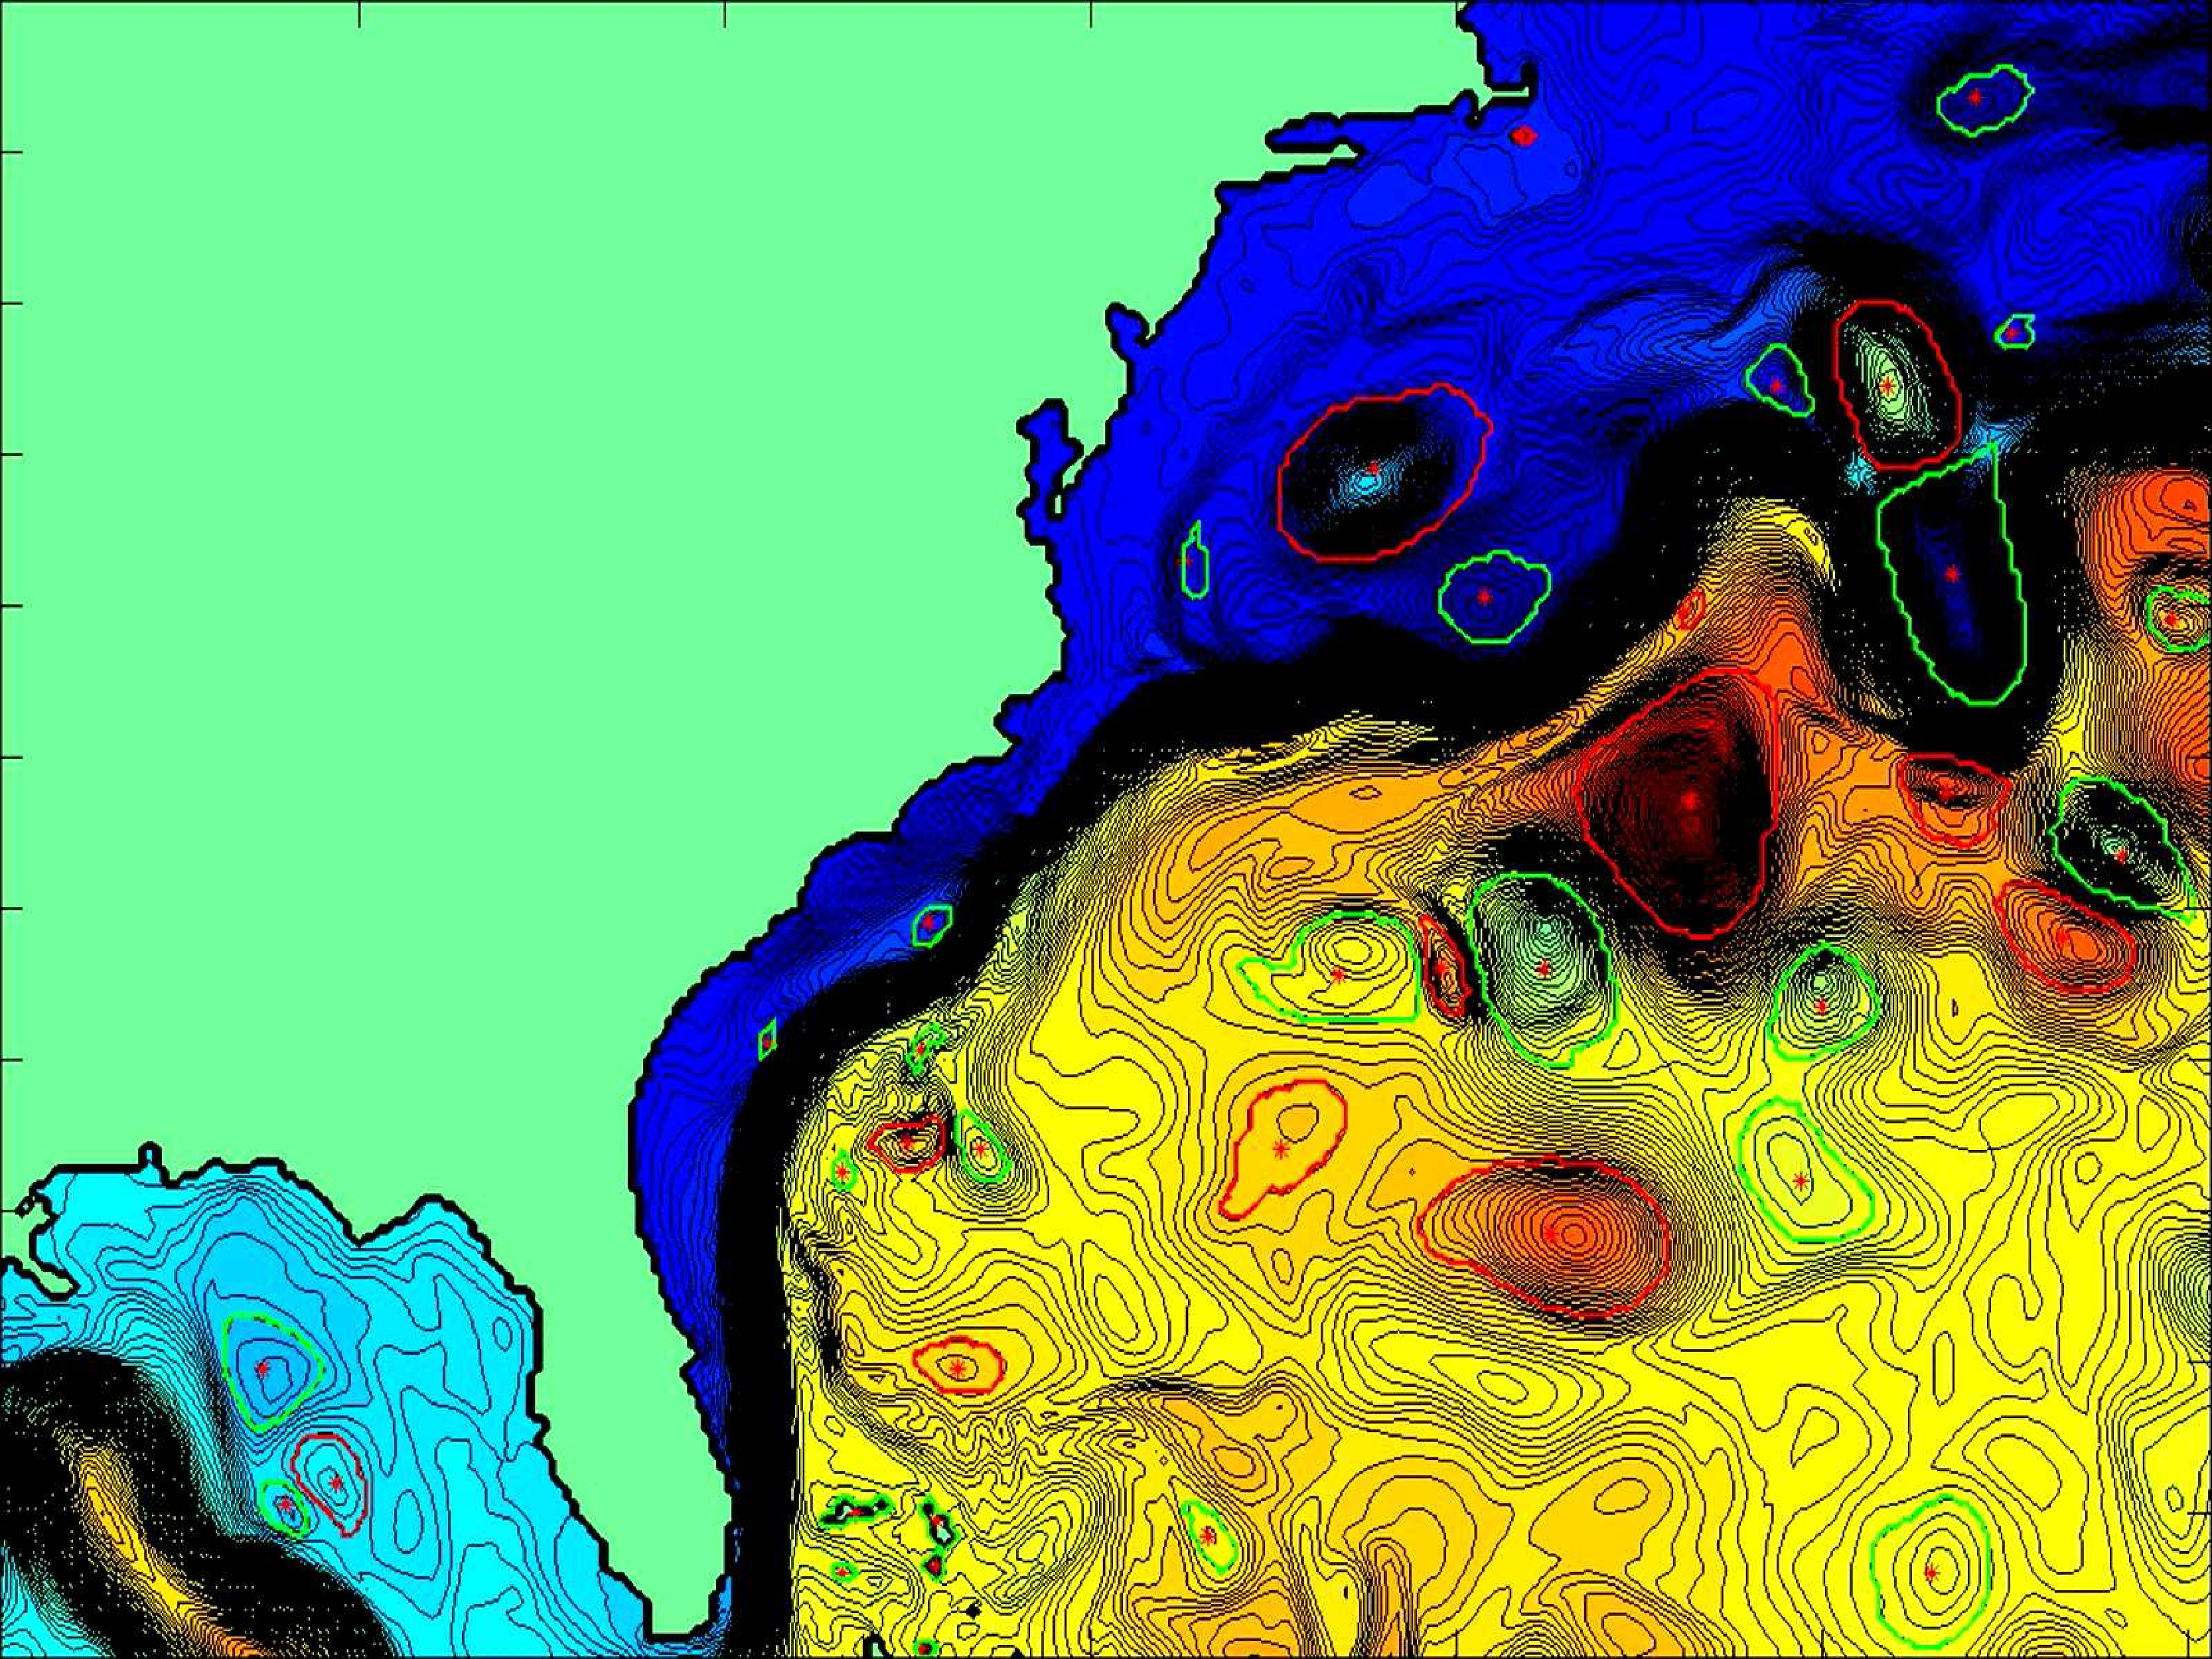
\includegraphics[width=300pt,keepaspectratio=true]{GS.pdf}
	%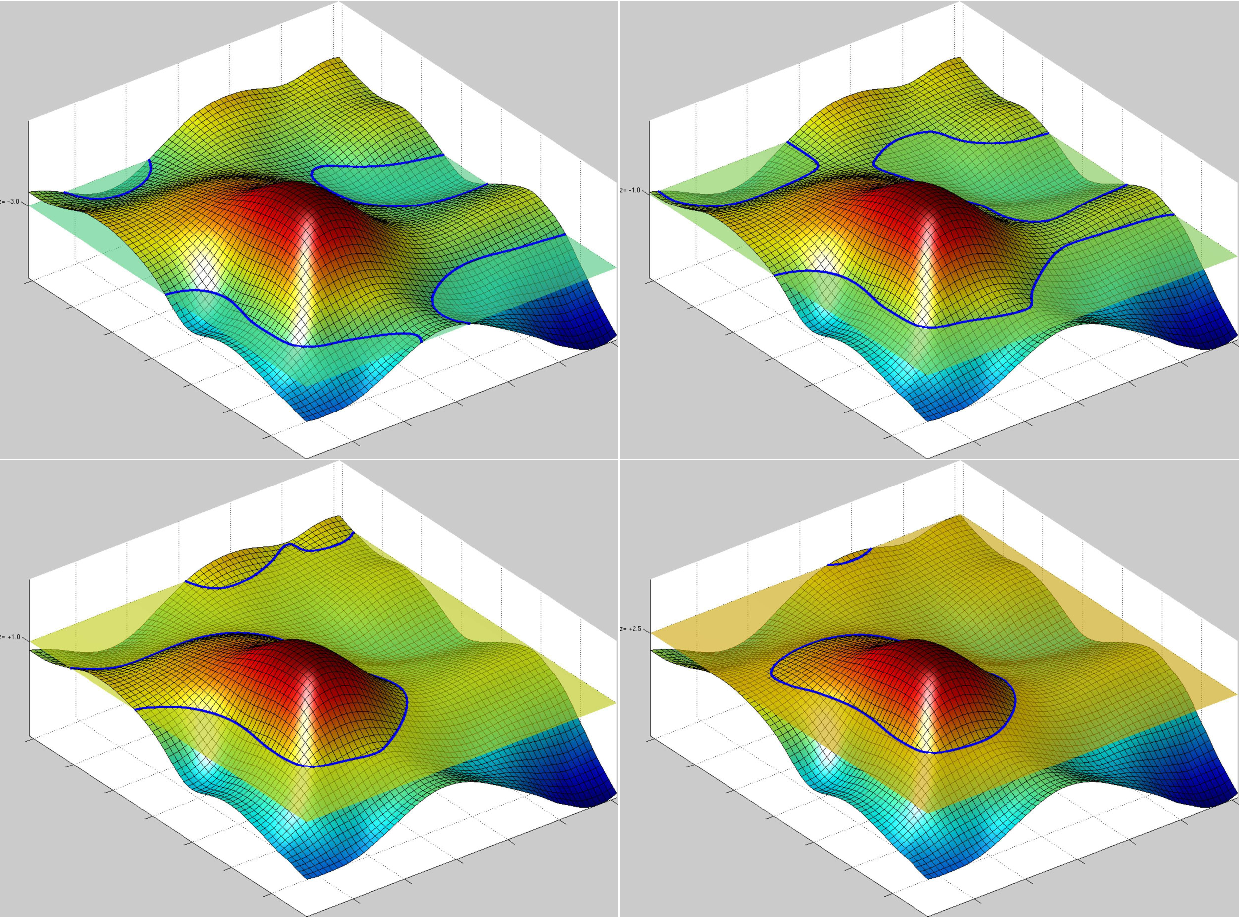
\includegraphics[height=200pt,keepaspectratio=true]{shrunks/sliceAll.pdf}
%\end{figure}
%\end{frame}

\begin{frame}
 \frametitle{does found contour qualify?}
\begin{figure}
	\begin{centering}
	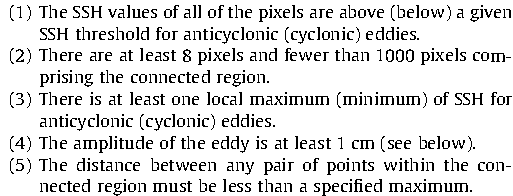
\includegraphics[width=.5\textwidth]{cheltCritsVerbatim.pdf}%
	\end{centering}
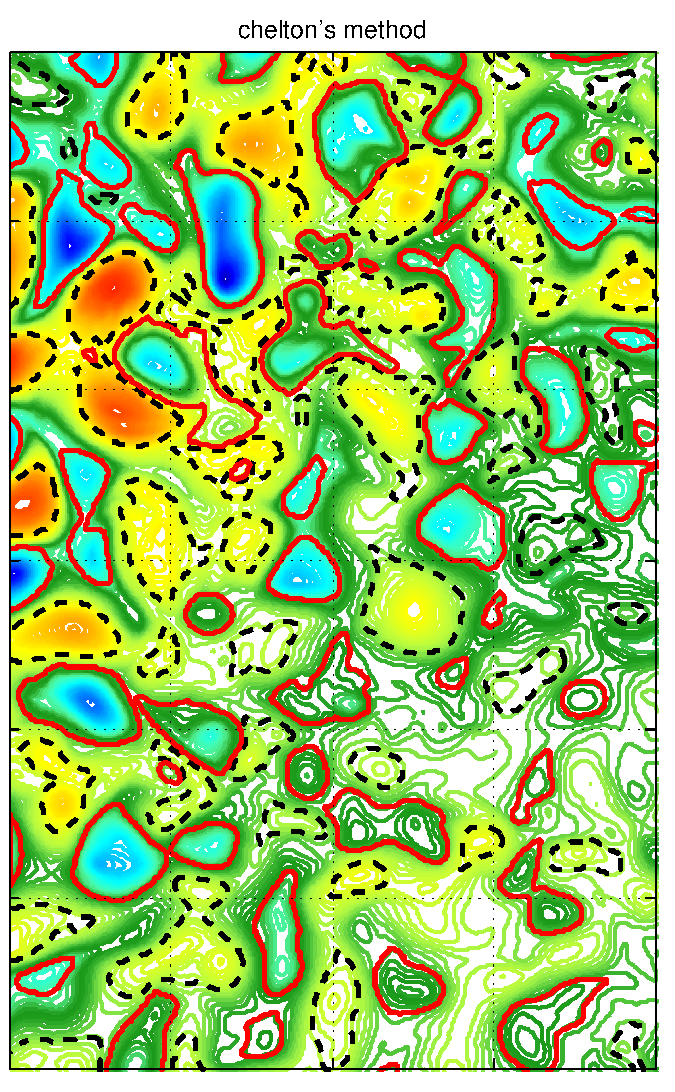
\includegraphics[height=200pt]{shrunks/ch.pdf}
\end{figure}
\end{frame}

\begin{frame}
 \frametitle{new approach: demand circular shapes}
\begin{figure}
%\includemovie{1cm}{1cm}{FIGS/Rotational_vortex.gif}
	\centering	
% 	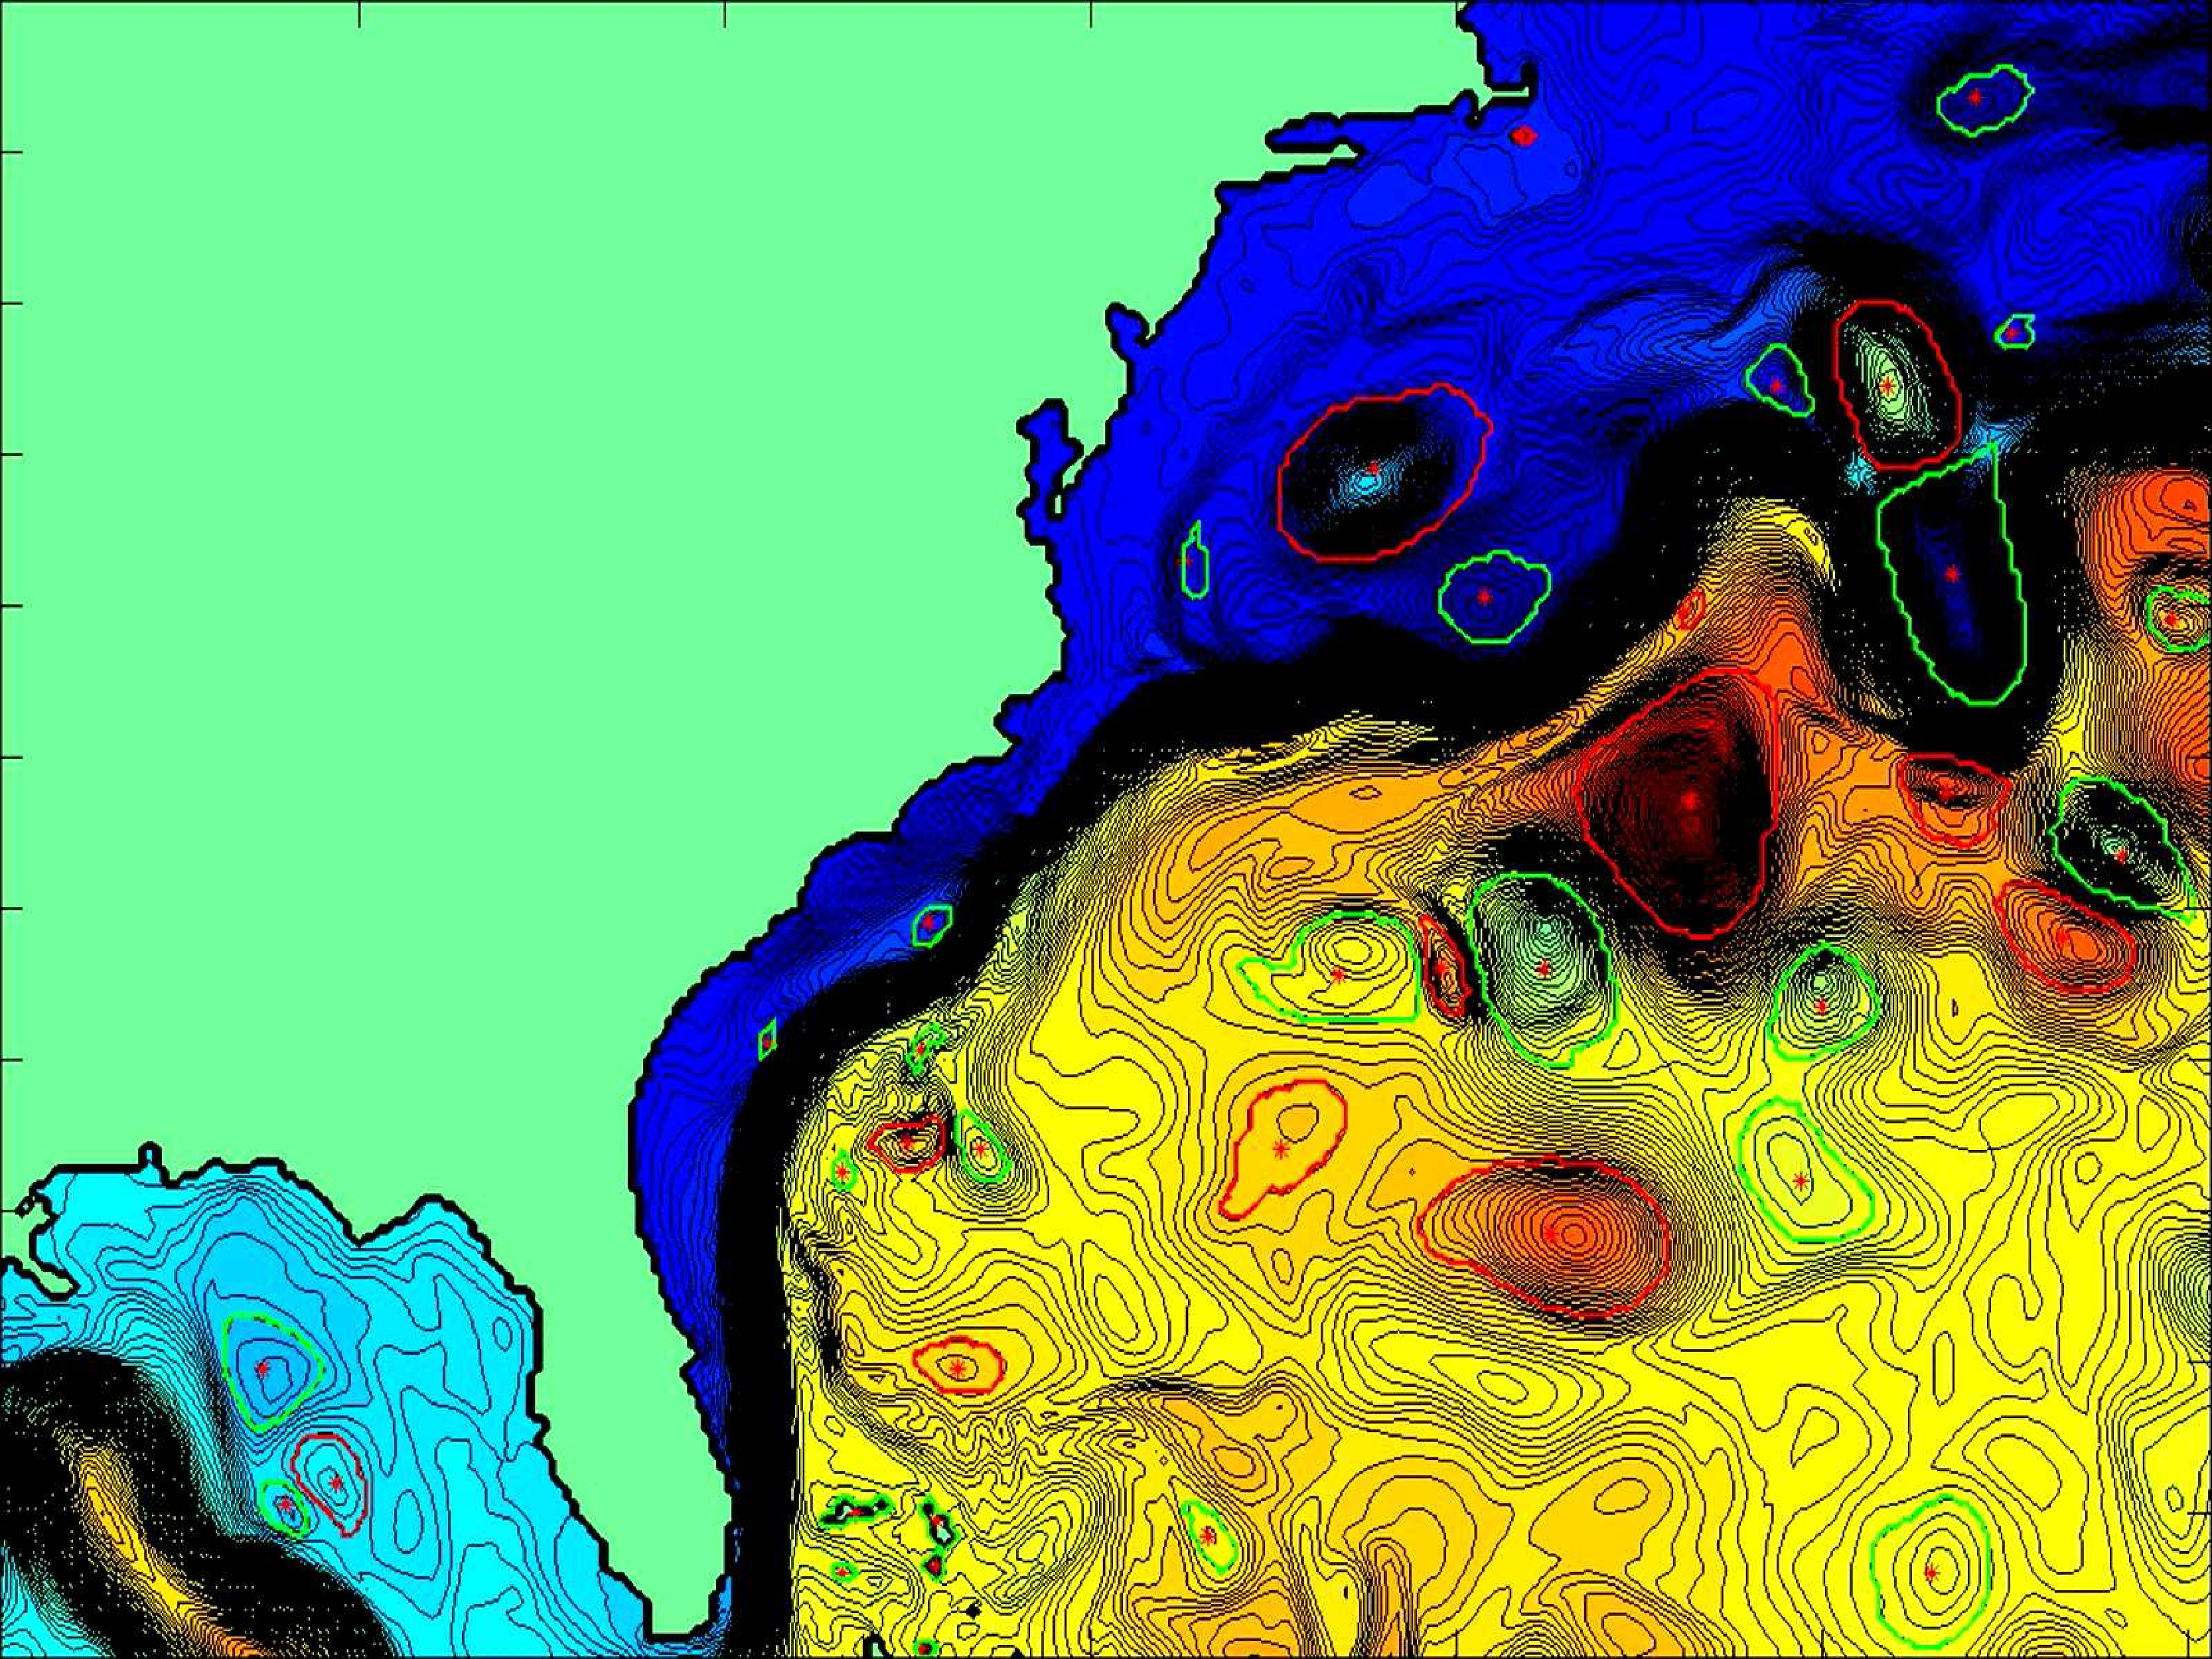
\includegraphics[width=300pt,keepaspectratio=true]{GS.pdf}
	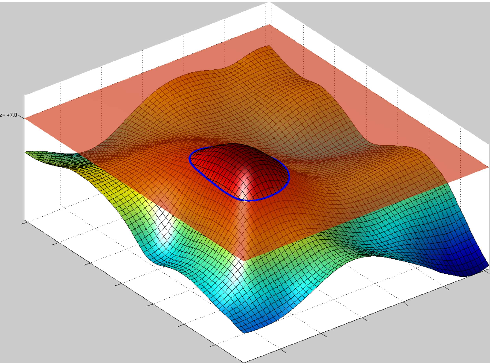
\includegraphics[height=200pt,keepaspectratio=true]{shrunks/slice5.pdf}
\end{figure}
\end{frame}

\begin{frame}
 %\frametitle{Isoperimetric Quotient (IQ): $A/A_{c}=\frac{A}{\pi r_{c}^{2}}=\frac{A}{\pi \left( \frac{c}{2\pi} \right)^{2}}=\frac{4 \pi A}{c}$}
 \frametitle{Isoperimetric Quotient}
  $IQ= A/A_{c}=\frac{4 \pi A}{c}$
\begin{figure}
	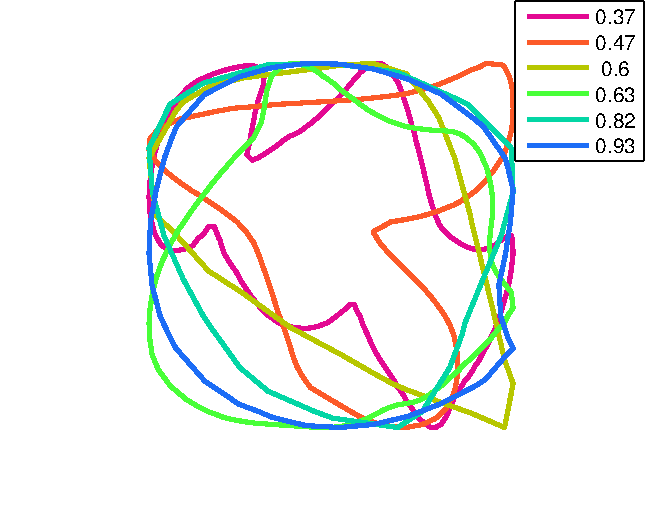
\includegraphics[height=150pt,keepaspectratio=true]{shrunks/isoper.pdf}
\end{figure}
\end{frame}

\begin{frame}
 \frametitle{new problem: deformed eddies get rejected}
\begin{figure}
	\centering
	%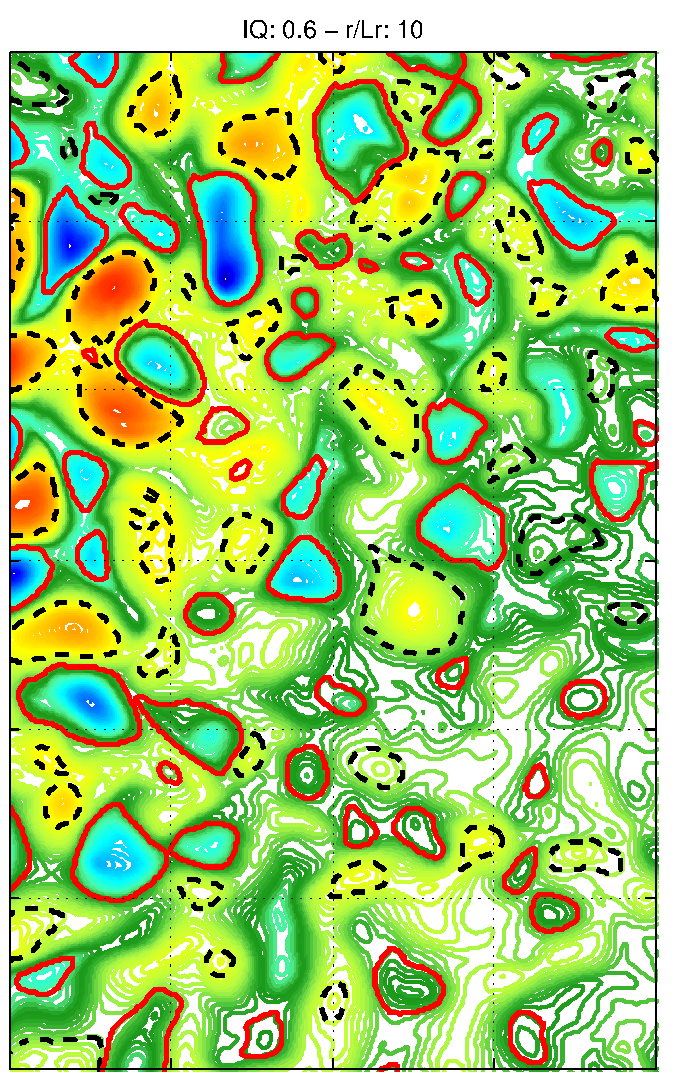
\includegraphics[height=200pt,keepaspectratio=true]{shrunks/iq6dlMrIc.pdf}
	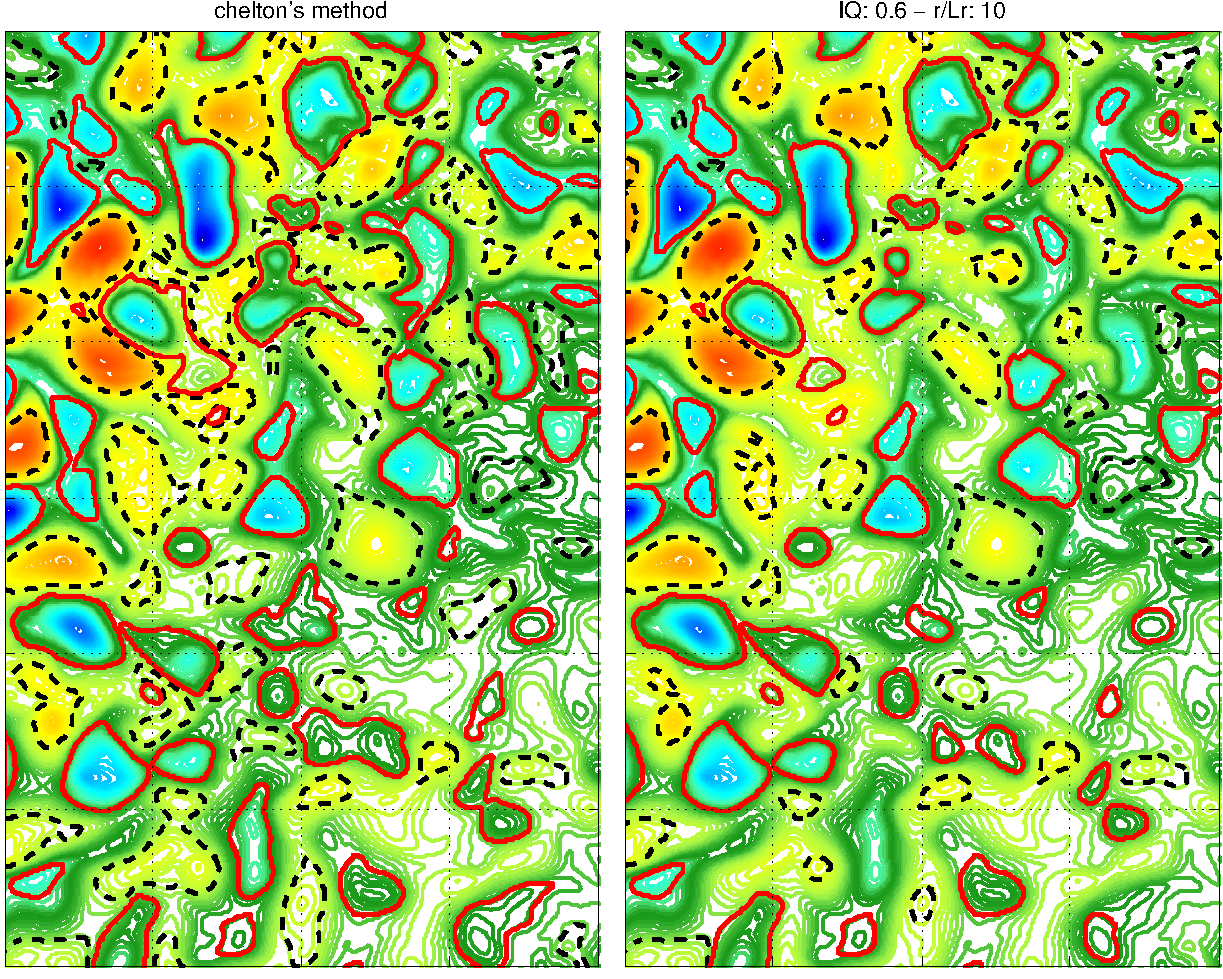
\includegraphics[height=200pt,keepaspectratio=true]{ch2iq6.pdf}
\end{figure}
\end{frame}


\begin{frame}
 \frametitle{solution: allow more deformation but limit hor. scale}
\begin{figure}
	\centering
% 	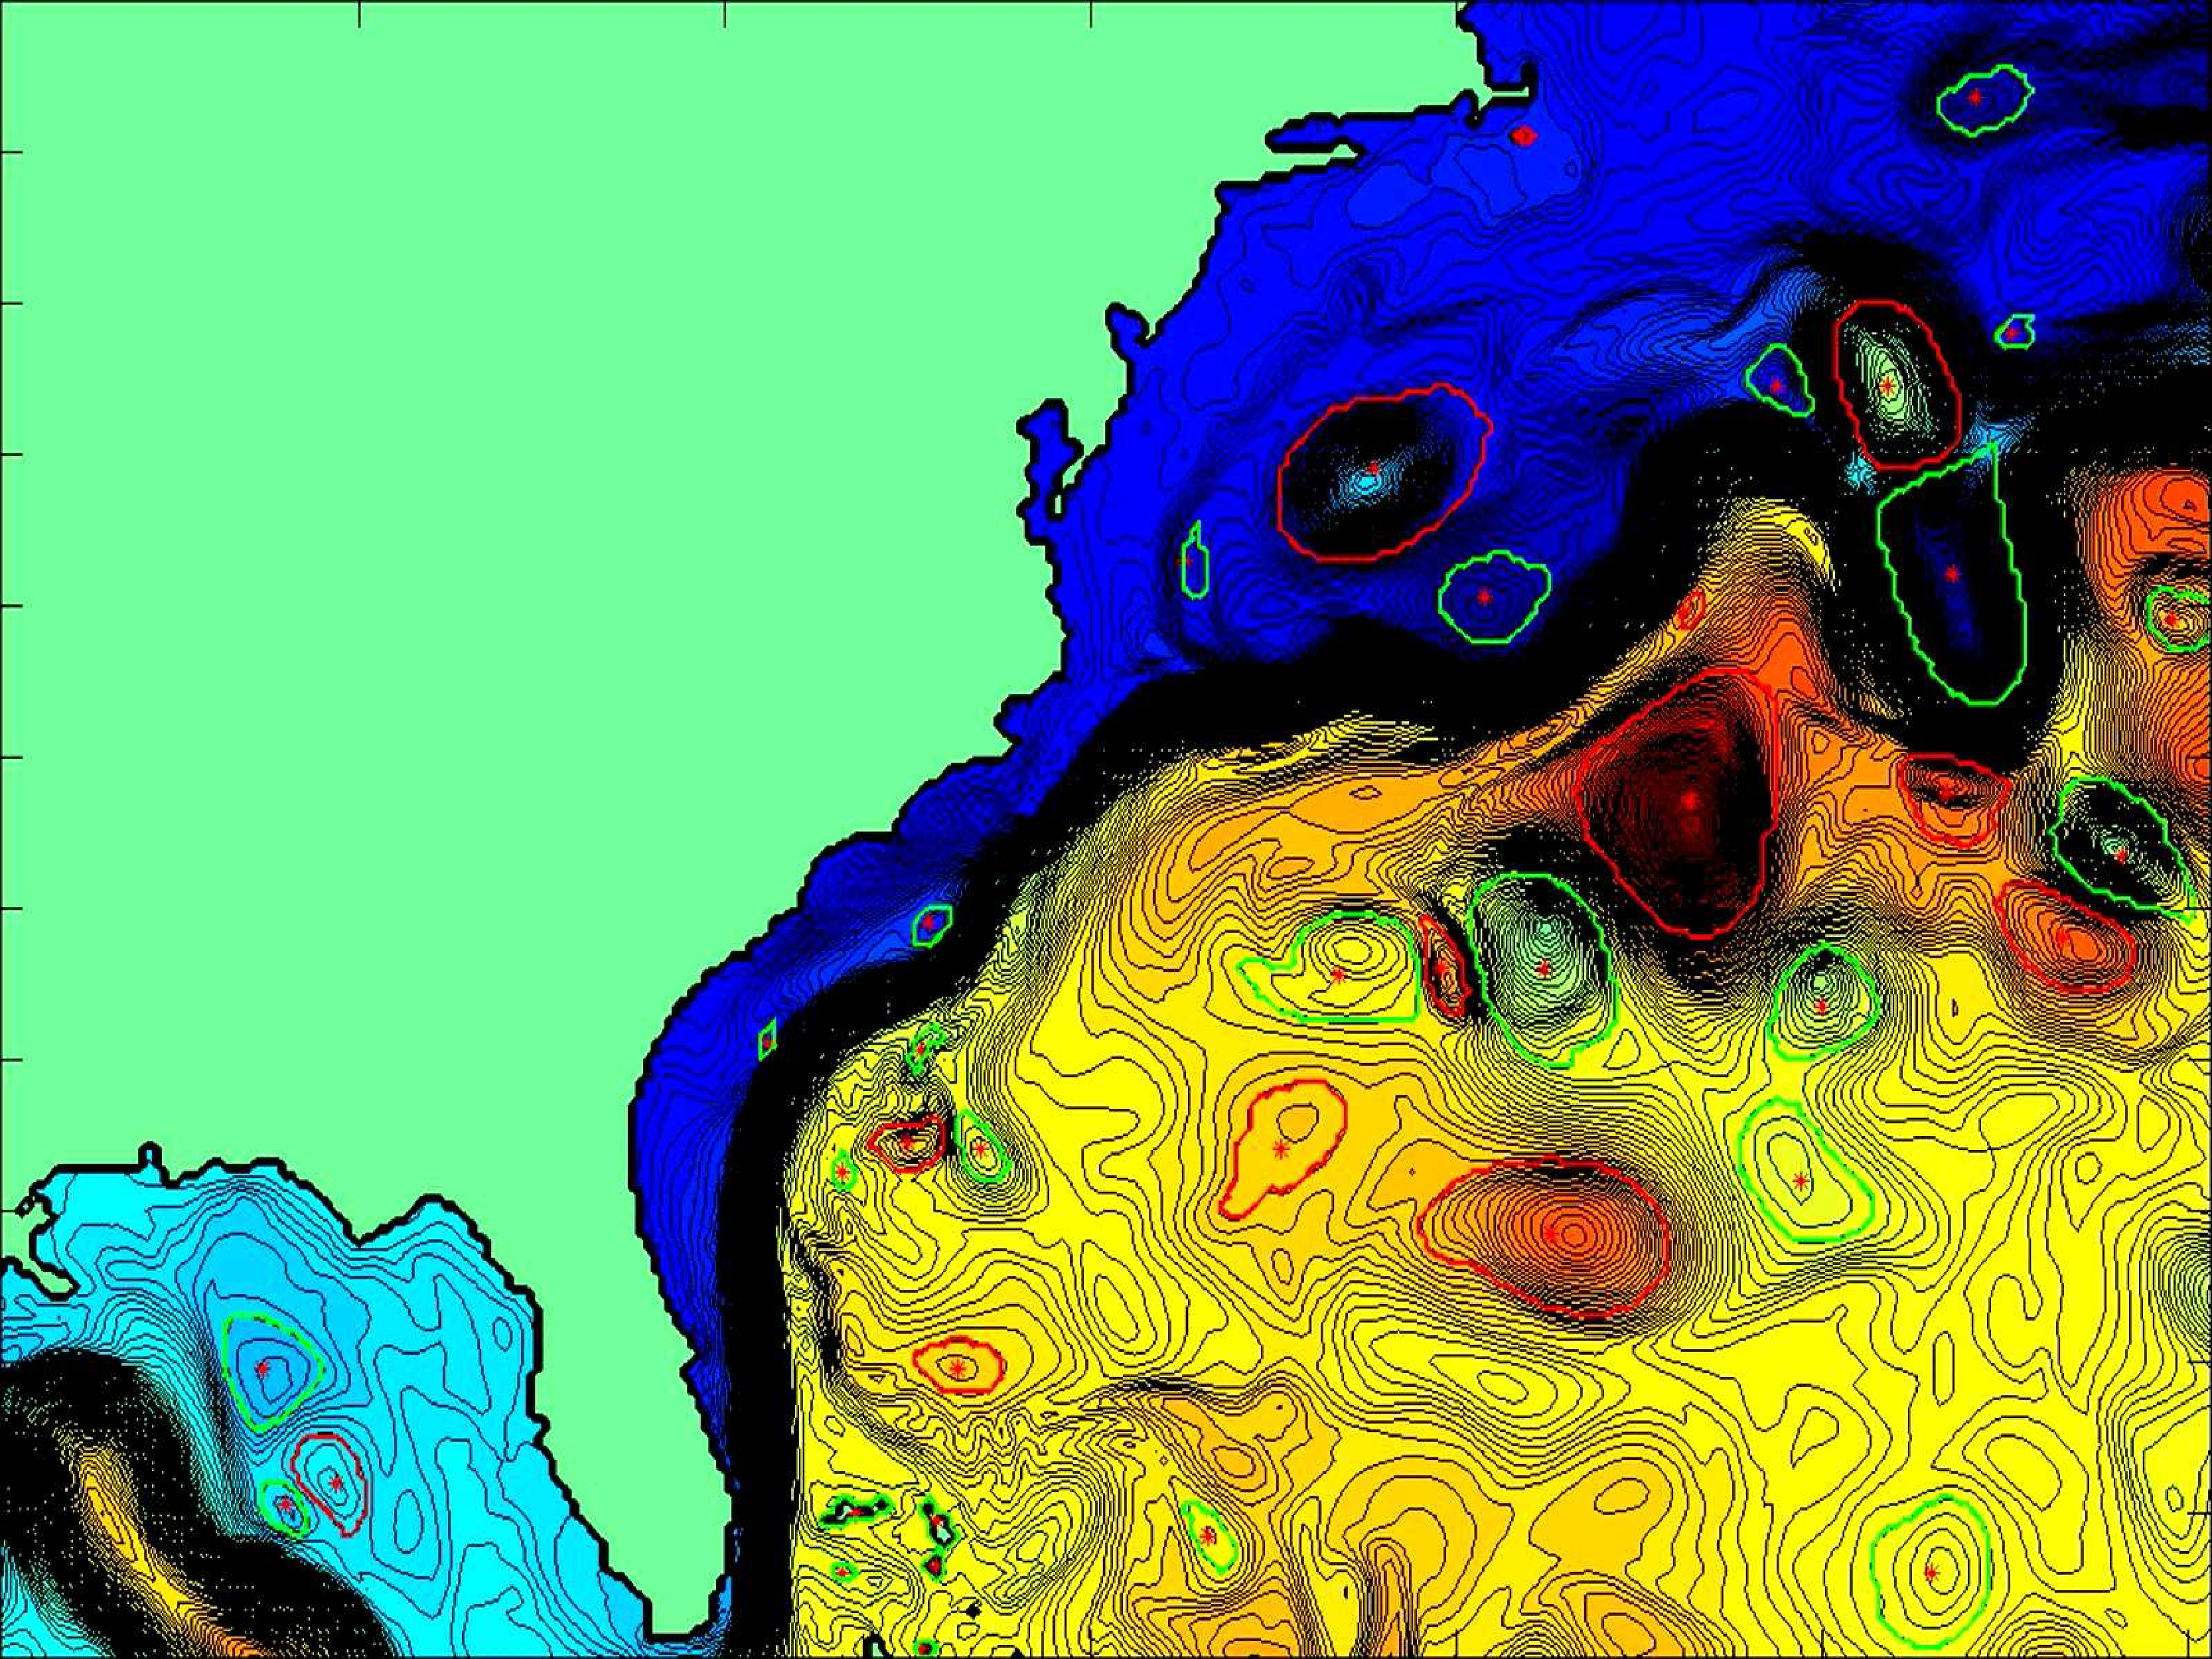
\includegraphics[width=300pt,keepaspectratio=true]{GS.pdf}
	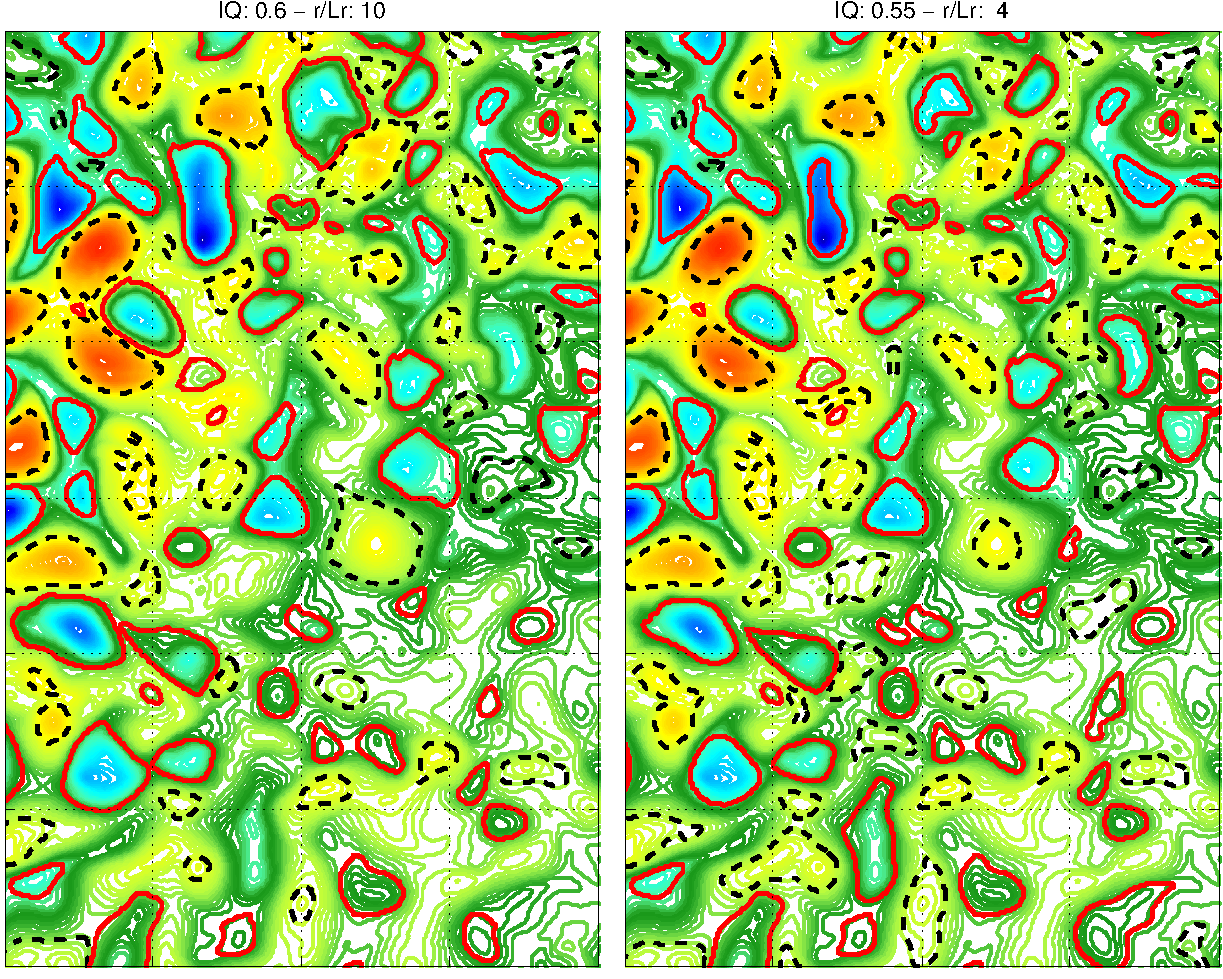
\includegraphics[height=200pt,keepaspectratio=true]{shrunks/iq6toiq55.pdf}
\end{figure}
\end{frame}

